\documentclass[11pt,aspectratio=169]{beamer}

\usepackage[utf8]{inputenc}
\usepackage[T1]{fontenc}
\usepackage[spanish,es-tabla]{babel}
\usepackage{lmodern}
\usepackage[table]{xcolor}
\usepackage{booktabs}
\usepackage{tikz}
\usetikzlibrary{positioning, arrows.meta, fit, shapes.geometric, calc, shadows.blur, backgrounds}
\usepackage[most]{tcolorbox}
\usepackage{listings}
\usepackage{microtype}
\usepackage{pifont}

% ============== Paleta ==============
\definecolor{accent}{HTML}{1F6FEB}
\definecolor{accent2}{HTML}{0A8754}
\definecolor{warn}{HTML}{D1351A}
\definecolor{bg}{HTML}{F6F8FA}
\definecolor{bgbox}{HTML}{EDF2F7}
\definecolor{rule}{HTML}{D0D7DE}
\definecolor{ink}{HTML}{1F2328}
\definecolor{muted}{HTML}{57606A}
\definecolor{good}{HTML}{1A7F37}

% ============== Tema beamer custom ==============
\usetheme{default}
\setbeamercolor{normal text}{fg=ink, bg=white}
\setbeamercolor{frametitle}{fg=accent, bg=white}
\setbeamercolor{title}{fg=ink}
\setbeamercolor{author}{fg=muted}
\setbeamercolor{date}{fg=muted}
\setbeamercolor{institute}{fg=muted}
\setbeamercolor{itemize item}{fg=accent}
\setbeamercolor{itemize subitem}{fg=accent}
\setbeamercolor{section in toc}{fg=ink}
\setbeamercolor{block title}{bg=bgbox, fg=accent}
\setbeamercolor{block body}{bg=bg, fg=ink}
\setbeamercolor{footline}{fg=muted}

\setbeamerfont{frametitle}{size=\Large, series=\bfseries}
\setbeamerfont{title}{size=\huge, series=\bfseries}

\setbeamertemplate{navigation symbols}{}
\setbeamertemplate{itemize item}{\raisebox{0.15ex}{\scriptsize\textbullet}}
\setbeamertemplate{itemize subitem}{\raisebox{0.1ex}{\scriptsize\textendash}}

% Frametitle con underline
\setbeamertemplate{frametitle}{%
  \nointerlineskip
  \vspace*{0.4em}
  \begin{beamercolorbox}[wd=\paperwidth, leftskip=0.6cm, rightskip=0.6cm]{frametitle}
    \insertframetitle\par
    \vspace*{0.15em}
    \textcolor{rule}{\rule{\dimexpr\paperwidth-1.2cm\relax}{0.4pt}}
  \end{beamercolorbox}
}

% Footline minimalista con ejercicio + slide num
\setbeamertemplate{footline}{%
  \leavevmode%
  \hbox{%
    \begin{beamercolorbox}[wd=0.5\paperwidth, ht=2.5ex, dp=1ex, leftskip=0.6cm]{footline}
      \usebeamerfont{footline}\small\insertshorttitle
    \end{beamercolorbox}%
    \begin{beamercolorbox}[wd=0.5\paperwidth, ht=2.5ex, dp=1ex, rightskip=0.6cm]{footline}
      \hfill\usebeamerfont{footline}\small\insertframenumber\,/\,\inserttotalframenumber
    \end{beamercolorbox}%
  }%
}

% ============== TCB blocks ==============
\newtcolorbox{insight}{
  enhanced, breakable,
  colback=bgbox, colframe=accent,
  boxrule=0pt, leftrule=4pt,
  arc=2pt, outer arc=0pt,
  left=8pt, right=8pt, top=4pt, bottom=4pt
}
\newtcolorbox{warning}{
  enhanced, breakable,
  colback=bgbox, colframe=warn,
  boxrule=0pt, leftrule=4pt,
  arc=2pt, outer arc=0pt,
  left=8pt, right=8pt, top=4pt, bottom=4pt
}
\newtcolorbox{takeaway}{
  enhanced, breakable,
  colback=accent2!8, colframe=accent2,
  boxrule=0pt, leftrule=4pt,
  arc=2pt, outer arc=0pt,
  left=8pt, right=8pt, top=4pt, bottom=4pt
}

% ============== JSON listings ==============
\definecolor{jsonkey}{HTML}{0550AE}
\definecolor{jsonstr}{HTML}{0A8754}
\lstdefinelanguage{json}{
    basicstyle=\ttfamily\scriptsize\color{ink},
    string=[s]{"}{"},
    stringstyle=\color{jsonstr},
    keywords={true,false,null},
    keywordstyle=\color{warn}\bfseries,
    showstringspaces=false,
    breaklines=true,
    backgroundcolor=\color{bg},
    frame=none,
    framexleftmargin=8pt,
    xleftmargin=8pt,
}

% ============== Custom commands ==============
\newcommand{\code}[1]{\texttt{\textcolor{accent}{#1}}}
\newcommand{\file}[1]{\texttt{\small #1}}
\newcommand{\ok}{\textcolor{good}{\ding{52}}}
\newcommand{\nok}{\textcolor{warn}{\ding{56}}}

% Section divider
\newcommand{\sectiondivider}[2]{%
  \begingroup
  \setbeamercolor{background canvas}{bg=accent}
  \begin{frame}[plain]
    \centering
    \vspace*{2cm}
    \color{white}
    {\fontsize{14}{16}\selectfont\bfseries Bloque #1}\\[1.2em]
    {\fontsize{32}{38}\selectfont\bfseries #2}\\[1.5em]
    \textcolor{white!75}{\rule{6cm}{0.4pt}}\\
  \end{frame}
  \endgroup
}

\title{TP3 — Perceptrones}
\subtitle{Implementación desde cero con NumPy}
\author{}
\institute{Sistemas de Inteligencia Artificial · ITBA · 1Q 2026}
\date{}
\titlegraphic{}

\setbeamertemplate{title page}{%
  \begin{tikzpicture}[remember picture, overlay]
    \fill[accent] (current page.north west) rectangle ($(current page.south west) + (0.5,0)$);
    \foreach \x in {0,...,28} {
      \foreach \y in {0,...,16} {
        \fill[accent!18] ($(current page.north west) + (1.0 + 0.5*\x, -0.6 - 0.5*\y)$) circle (1pt);
      }
    }
  \end{tikzpicture}
  \vspace*{1.4cm}
  \begin{flushleft}
    \hspace*{1cm}{\fontsize{40}{46}\selectfont\bfseries\color{ink}TP3}\\[0.3em]
    \hspace*{1cm}{\fontsize{30}{36}\selectfont\bfseries\color{accent}Perceptrones}\\[0.6em]
    \hspace*{1cm}{\Large\color{muted}\inserttitle\hfill}\\
    \hspace*{1cm}{\large\color{muted}\insertsubtitle}\\[1.6em]
    \hspace*{1cm}{\color{muted}\insertinstitute}\\
  \end{flushleft}
}

% ===================================================================
\begin{document}

% ============= 1. Portada =============
{
\setbeamertemplate{footline}{}
\begin{frame}[plain]
  \titlepage
\end{frame}
}

% ===================================================================
% PERSONA 1
% ===================================================================
\sectiondivider{1 / 4}{Introducción + Engine + Validación}

% ============= 2. Qué pide el TP =============
\begin{frame}{Qué pide el TP}
\textbf{Tres ejercicios + validación, todo desde cero en NumPy.}\\[0.6em]

\begin{tabular}{@{}p{0.18\linewidth}p{0.78\linewidth}@{}}
\toprule
\textbf{Ej 0}    & Validación: AND (step), XOR (MLP), lineal y tanh \\
\midrule
\textbf{Ej 1}    & Detección de fraude por \emph{knowledge distillation} \\
\midrule
\textbf{Ej 2}    & Clasificación de dígitos manuscritos (MLP, 10 clases) \\
\midrule
\textbf{Ej 3}    & Lo mismo que Ej 2, target: \textbf{accuracy $\geq 98\%$} \\
\bottomrule
\end{tabular}\\[1em]

\begin{warning}
\textbf{Restricción explícita del enunciado:} sin sklearn estimators, sin PyTorch ni TensorFlow como capas. Solo NumPy para matrices, Pandas para datos, Matplotlib para plots.
\end{warning}
\end{frame}

% ============= 3. Arquitectura del repo =============
\begin{frame}[fragile]{Filosofía: un engine, muchos configs}
\begin{columns}[T]
\column{0.5\linewidth}
\textbf{Decisión arquitectural:}\\
Módulo \code{mlp/} reutilizable + configs JSON.\\[0.6em]

\textbf{Beneficios:}
\begin{itemize}
  \item Una codebase, 78 tests verde
  \item Cambiar de Ej0 a Ej3 = cambiar de JSON
  \item Pack C del Ej3 = 3 líneas en \code{regularization}
\end{itemize}

\column{0.5\linewidth}
\begin{lstlisting}[language=bash, basicstyle=\ttfamily\scriptsize\color{ink},
                   backgroundcolor=\color{bg}, frame=none, framexleftmargin=8pt,
                   xleftmargin=8pt]
mlp/                  <- engine (NumPy)
ejercicio0/           <- AND, XOR, validacion
ejercicio1/           <- fraud (Tomas, scripts aparte)
ejercicio2/           <- digitos
ejercicio3/           <- digitos >= 98%
docs/                 <- specs, plans, guias
\end{lstlisting}
\end{columns}
\end{frame}

% ============= 4. Anatomía del engine =============
\begin{frame}{Anatomía del engine \code{mlp/}}
\centering
\begin{tikzpicture}[
    every node/.style={font=\footnotesize},
    block/.style={
      draw=accent, fill=bg, rounded corners=2pt,
      minimum width=2.6cm, minimum height=0.7cm
    },
    cmp/.style={
      draw=accent2, fill=accent2!10, rounded corners=2pt,
      minimum width=2.6cm, minimum height=0.6cm
    },
    arrow/.style={-{Latex[length=2mm]}, accent, thick}
]
  \node[block] (forward) {\code{forward(X, training)}};
  \node[block, below=0.3cm of forward] (backward) {\code{backward(X, y, cache)}};
  \node[block, below=0.3cm of backward] (fit) {\code{fit / predict}};

  \node[cmp, right=2.0cm of forward, yshift=0.3cm] (act) {Activations};
  \node[cmp, below=0.18cm of act] (loss) {Losses};
  \node[cmp, below=0.18cm of loss] (init) {Initializers};
  \node[cmp, below=0.18cm of init] (opt) {Optimizers};

  \draw[arrow] (forward) -- (backward);
  \draw[arrow] (backward) -- (fit);

  \draw[arrow, dashed, opacity=0.6] (act.west) -- ++(-0.6,0) |- (forward.east);
  \draw[arrow, dashed, opacity=0.6] (loss.west) -- ++(-0.6,0) |- (backward.east);
  \draw[arrow, dashed, opacity=0.6] (init.west) -- ++(-0.6,0) |- ($(forward.east)+(0,-0.1)$);
  \draw[arrow, dashed, opacity=0.6] (opt.west) -- ++(-0.6,0) |- (fit.east);

  \node[font=\bfseries\color{accent}, above=0.05cm of forward] {Pipeline};
  \node[font=\bfseries\color{accent2}, above=0.05cm of act] {Componentes};
\end{tikzpicture}\\[0.5em]

\small
\begin{tabular}{@{}lll@{}}
\toprule
Activaciones & Losses & Optimizadores \\
\midrule
sigmoid, tanh, relu, identity, softmax & MSE, BCE, cross\_entropy & SGD, Momentum, Adam \\
\bottomrule
\end{tabular}\\[0.4em]

\textcolor{muted}{\footnotesize Bias trick: cada $W^{(l)}$ tiene shape $(n_{l+1},\, n_l + 1)$, columna 0 es bias.}
\end{frame}

% ============= 5. Ej0 AND =============
\begin{frame}[fragile]{Ej 0 — AND con perceptrón escalón}
\begin{columns}[T]
\column{0.55\linewidth}
\textbf{Representación bipolar (apunte)}: entradas $\{-1, +1\}$, salida esperada $[-1, -1, -1, +1]$.\\[0.4em]

Update con función signo:
\[
\Delta w = \eta\,(z - O)\,x \quad \text{con } O = \mathrm{sign}(w \cdot x)
\]

\textbf{Test:} converge a error $=0$ en pocas epochs. Implementación en \file{ejercicio0/step\_perceptron.py}.

\column{0.45\linewidth}
\begin{lstlisting}[language=json, basicstyle=\ttfamily\scriptsize]
{
  "loss": "mse",
  "optimizer": {"name":"sgd","lr":0.1},
  "activations": ["step"],
  "epochs": 100
}
\end{lstlisting}
\vspace{0.4em}
\begin{insight}
\small Validación pre-engine: si AND no converge, hay un bug en la pipeline.
\end{insight}
\end{columns}
\end{frame}

% ============= 6. Ej0 XOR =============
\begin{frame}{Ej 0 — XOR como red de seguridad}
\textbf{XOR no es separable linealmente.} Necesita capa oculta no-lineal.\\[0.4em]

Probamos dos arquitecturas:
\begin{itemize}
  \item $[2, 2, 1]$ — la mínima que resuelve XOR (configs/xor\_2\_2\_1.json)
  \item $[2, 3, 2, 1]$ — con capa extra para validar arquitecturas profundas
\end{itemize}

\vspace{0.4em}
\begin{takeaway}
\textbf{XOR es la red de seguridad del engine.}\\
Durante el desarrollo encontramos 4 bugs reales que se manifestaban acá antes que en dígitos:
\begin{itemize}
  \item \code{predict()} devolvía $\{0,1\}$ en vez de $\{-1,+1\}$ para tanh-binario.
  \item \code{identity} activation aliasaba su input.
  \item \code{numerical\_grad} con int dtype daba garbage silencioso.
  \item Mean/std del run\_summary perdía strings por dict-spread overwrite.
\end{itemize}
\end{takeaway}
\end{frame}

% ===================================================================
% PERSONA 2 — TOMÁS
% ===================================================================
\sectiondivider{2 / 4}{Ej 1 — Knowledge Distillation}

% ============= 7. Setup Ej1 =============
\begin{frame}{Ej 1 — El problema}
\textbf{Knowledge distillation:} replicar la salida de un BigModel pre-entrenado con un TinyModel (perceptrón simple).\\[0.6em]

\begin{columns}[T]
\column{0.55\linewidth}
\textbf{Datos:} \file{fraud\_dataset.csv}\\
9 features (timestamp, amount, session\ldots)\\[0.4em]

\textbf{Target de entrenamiento:}\\
\code{big\_model\_fraud\_probability} (continuo en $[0,1]$)\\[0.4em]

\textbf{Ground truth de evaluación:}\\
\code{flagged\_fraud} (binaria)

\column{0.45\linewidth}
\begin{warning}
\textbf{Regla del enunciado:} \code{flagged\_fraud} \emph{nunca} se usa para entrenar. Solo para métricas operativas (precision/recall/F1) post-hoc.
\end{warning}\\[0.6em]

\textbf{Salida en $[0,1]$} $\Rightarrow$ activación sigmoide.
\end{columns}
\end{frame}

% ============= 8. Features y código =============
\begin{frame}[fragile]{Ej 1 — Setup técnico}
\textbf{Pipeline:} K-fold estratificado por \code{flagged\_fraud}, normalización z-score \emph{fit-on-train-only} (sin leakage), online learning sample-by-sample.\\[0.4em]

\textbf{Features excluidas} (3 de 12 columnas): \code{timestamp}, \code{device\_screen\_resolution}, \code{time\_since\_last\_login\_s}.\\[0.4em]

\begin{lstlisting}[language=json, basicstyle=\ttfamily\scriptsize]
// ejercicio1/nonlinear_perceptron/configs/baseline.json
{
  "target_col": "big_model_fraud_probability",
  "eval_col":   "flagged_fraud",
  "exclude_features": ["timestamp", "device_screen_resolution",
                        "time_since_last_login_s"],
  "k_folds": 5,
  "stratify": true,
  "training": {"learning_rate": 0.0001, "epochs": 500, "epsilon": 1e-5},
  "evaluation": {"threshold": 0.5},
  "normalization": "zscore"
}
\end{lstlisting}
\end{frame}

% ============= 9. Lineal vs No-Lineal =============
\begin{frame}{Ej 1 — Lineal vs No-Lineal}
\begin{columns}[T]
\column{0.5\linewidth}
\textbf{Lineal (Adaline)}\\
\[ O = w \cdot x \]
\[ \Delta w = \eta\,(z - O)\,x \]

\column{0.5\linewidth}
\textbf{No-Lineal (Sigmoide)}\\
\[ O = \sigma(w \cdot x) \]
\[ \Delta w = \eta\,(z - O)\,O(1-O)\,x \]
\end{columns}
\vspace{0.6em}

\textcolor{muted}{El factor $O(1-O)$ modula el gradiente: se achica en zonas saturadas (cerca de 0 o 1), es máximo cerca de 0.5.}\\[0.6em]

\centering
\begin{tabular}{@{}lr@{}}
\toprule
\textbf{Modelo} & \textbf{MSE test (mean $\pm$ std)} \\
\midrule
Lineal     & $0.0266 \pm 0.0008$ \\
\rowcolor{accent2!15}
\textbf{No-Lineal} & $\boldsymbol{0.0110 \pm 0.0004}$ \quad ($\boldsymbol{-59\%}$) \\
\bottomrule
\end{tabular}
\end{frame}

% ============= 10. Por qué sigmoide gana =============
\begin{frame}[fragile]{Ej 1 — Por qué la sigmoide gana}
\begin{insight}
\textbf{El target está acotado en $[0,1]$.} La sigmoide mapea naturalmente al rango del target. El lineal puede producir valores fuera del rango y el MSE lo penaliza fuerte.
\end{insight}
\vspace{0.6em}

\textbf{Implementación con estabilidad numérica}: la sigmoide del código de Tomás usa máscara para evitar overflow en \code{exp}:
\begin{lstlisting}[language=python, basicstyle=\ttfamily\scriptsize\color{ink},
                   backgroundcolor=\color{bg}, frame=none,
                   framexleftmargin=8pt, xleftmargin=8pt]
def sigmoid(x):
    out = np.empty_like(x)
    pos = x >= 0
    out[pos]  = 1.0 / (1.0 + np.exp(-x[pos]))
    exp_x = np.exp(x[~pos])
    out[~pos] = exp_x / (1.0 + exp_x)
    return out
\end{lstlisting}
\end{frame}

% ============= 11. Threshold default es engañoso =============
\begin{frame}{Ej 1 — El threshold default es engañoso}
\textbf{Con threshold = 0.5:} precision = 0.33, recall = 1.00.\\
Casi todo se clasifica como fraude. \textbf{Pero el modelo no es malo} — el threshold está mal.\\[0.6em]

\begin{insight}
Las salidas sigmoide se concentran: la mediana de los scores de fraude está en \textbf{0.99}. Los no-fraudes tampoco bajan a 0.05; bajan a 0.4--0.6. El modelo aprendió ranking, no calibración.
\end{insight}
\vspace{0.6em}

\textbf{Solución:} barrer el threshold de 0.00 a 1.00, paso 0.01.
\end{frame}

% ============= 12. Threshold óptimo =============
\begin{frame}{Ej 1 — Threshold sweep}
\centering
\small
\begin{tabular}{@{}rcccc@{}}
\toprule
\textbf{Threshold} & \textbf{Precision} & \textbf{Recall} & \textbf{F1} & \textbf{Accuracy} \\
\midrule
0.50 & 0.333 & 1.000 & 0.499 & 0.768 \\
0.80 & 0.751 & 0.952 & 0.840 & 0.958 \\
0.85 & 0.812 & 0.893 & 0.850 & 0.964 \\
\rowcolor{accent2!15}
\textbf{0.89} & \textbf{0.886} & \textbf{0.861} & \textbf{0.873} & \textbf{0.971} \\
0.95 & 0.949 & 0.746 & 0.835 & 0.966 \\
0.99 & 1.000 & 0.527 & 0.690 & 0.945 \\
\bottomrule
\end{tabular}\\[0.8em]

\textbf{AUC-ROC:} no-lineal \(0.9921\)\quad vs\quad lineal \(0.9720\).\\[0.8em]

\begin{takeaway}
\textbf{Recomendación:} threshold \(=0.89\) si se prioriza F1; \(\geq 0.95\) si los falsos positivos son costosos. Decisión de negocio sobre el costo asimétrico FN/FP.
\end{takeaway}
\end{frame}

% ===================================================================
% PERSONA 3
% ===================================================================
\sectiondivider{3 / 4}{Ej 2 — Clasificación de dígitos}

% ============= 13. Problema Ej2 =============
\begin{frame}{Ej 2 — El problema}
\textbf{Clasificación multiclase de dígitos manuscritos (0--9).}\\[0.6em]

\begin{columns}[T]
\column{0.5\linewidth}
\textbf{Datos:}
\begin{itemize}
  \item Train: \file{digits.csv} (12.449 muestras)
  \item Test: \file{digits\_test.csv} (2.498)
\end{itemize}
Cada muestra: vector de 784 floats $\in [0,1]$ (28$\times$28 flatten).

\column{0.5\linewidth}
\textbf{Arquitectura final:}
\begin{itemize}
  \item Input: 784
  \item Hidden 1: 100 (ReLU)
  \item Hidden 2: 50 (ReLU)
  \item Output: 10 (Softmax)
\end{itemize}
\end{columns}
\vspace{0.6em}

\begin{warning}
\textbf{Regla:} \code{digits\_test.csv} se evalúa una sola vez, al final. No se toca durante búsqueda de hiperparámetros.
\end{warning}
\end{frame}

% ============= 14. Workflow Fase 1+2 =============
\begin{frame}{Ej 2 — Workflow disciplinado}
\centering
\begin{tikzpicture}[
  every node/.style={font=\small},
  phase/.style={
    draw=accent, fill=bg, rounded corners=3pt,
    minimum width=3.4cm, minimum height=1.4cm, align=center
  },
  result/.style={
    draw=accent2, fill=accent2!10, rounded corners=3pt,
    minimum width=3.4cm, minimum height=1.4cm, align=center
  },
  arrow/.style={-{Latex[length=3mm]}, accent, very thick}
]
  \node[phase] (f1) {\textbf{Fase 1}\\\footnotesize k\_folds=1\\\footnotesize arch \(\to\) opt \(\to\) LR \(\to\) batch};
  \node[result, right=1.2cm of f1] (base) {\textbf{base.json}\\\footnotesize ganador\\\footnotesize consolidado};
  \node[phase, right=1.2cm of base] (f2) {\textbf{Fase 2}\\\footnotesize k\_folds=5\\\footnotesize one-at-a-time};
  \node[result, below=0.6cm of base] (final) {\textbf{final\_eval}\\\footnotesize digits\_test.csv\\\footnotesize (UNA sola vez)};

  \draw[arrow] (f1) -- (base);
  \draw[arrow] (base) -- (f2);
  \draw[arrow] (f2.south) -- ++(0,-0.3) -| (final.east);
  \draw[arrow, dashed] (base.south) -- (final.north);
\end{tikzpicture}\\[0.6em]

\begin{insight}
\textbf{Reduce $\mathcal{O}(n^4)$ a $\mathcal{O}(4n)$.} Sweeps secuenciales en Fase 1; one-at-a-time en Fase 2 valida la elección con K=5.
\end{insight}
\end{frame}

% ============= 15. Ganadores Fase 1 =============
\begin{frame}{Ej 2 — Ganadores de Fase 1}
\centering
\small
\begin{tabular}{@{}llrl@{}}
\toprule
\textbf{Sub-fase} & \textbf{Ganador} & \textbf{val\_acc} & \textbf{Comentario} \\
\midrule
1.1 Arquitectura  & $[784,100,50,10]$ & 0.9674 & Empate técnico, parsimonia \\
1.2 Optimizador   & adam (lr=0.001)   & 0.9674 & SGD no convergió en 50 ep \\
1.3 Learning rate & 0.001             & 0.9674 & 0.0001 lento, $\geq 0.005$ overshoot \\
1.4 Batch size    & 16                & 0.9674 & best\_ep=3, el más rápido \\
\bottomrule
\end{tabular}\\[0.8em]

\textbf{\code{base.json} consolidado, K-fold=5:}\\
\begin{center}\Large
val\_acc = $\boldsymbol{0.9622 \pm 0.0043}$
\end{center}
\end{frame}

% ============= 16. Plots Fase 2 =============
\begin{frame}{Ej 2 — Fase 2 valida la elección}
\centering
\begin{columns}[T]
\column{0.5\linewidth}
\centering
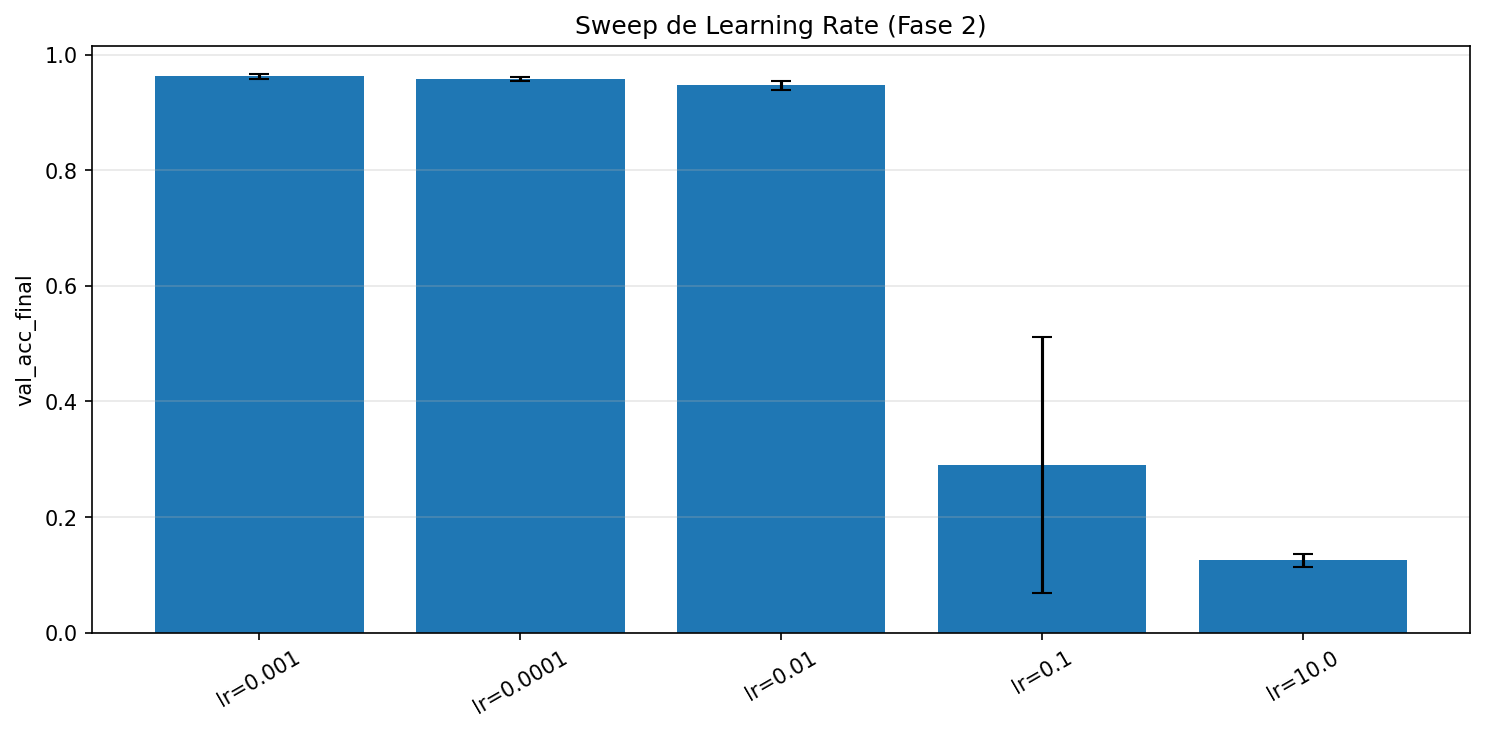
\includegraphics[width=\linewidth]{../ejercicio2/presentacion/02_sweep_lr.png}\\
\textcolor{muted}{\footnotesize Sweep LR — \code{lr=10} es accuracy random}
\column{0.5\linewidth}
\centering
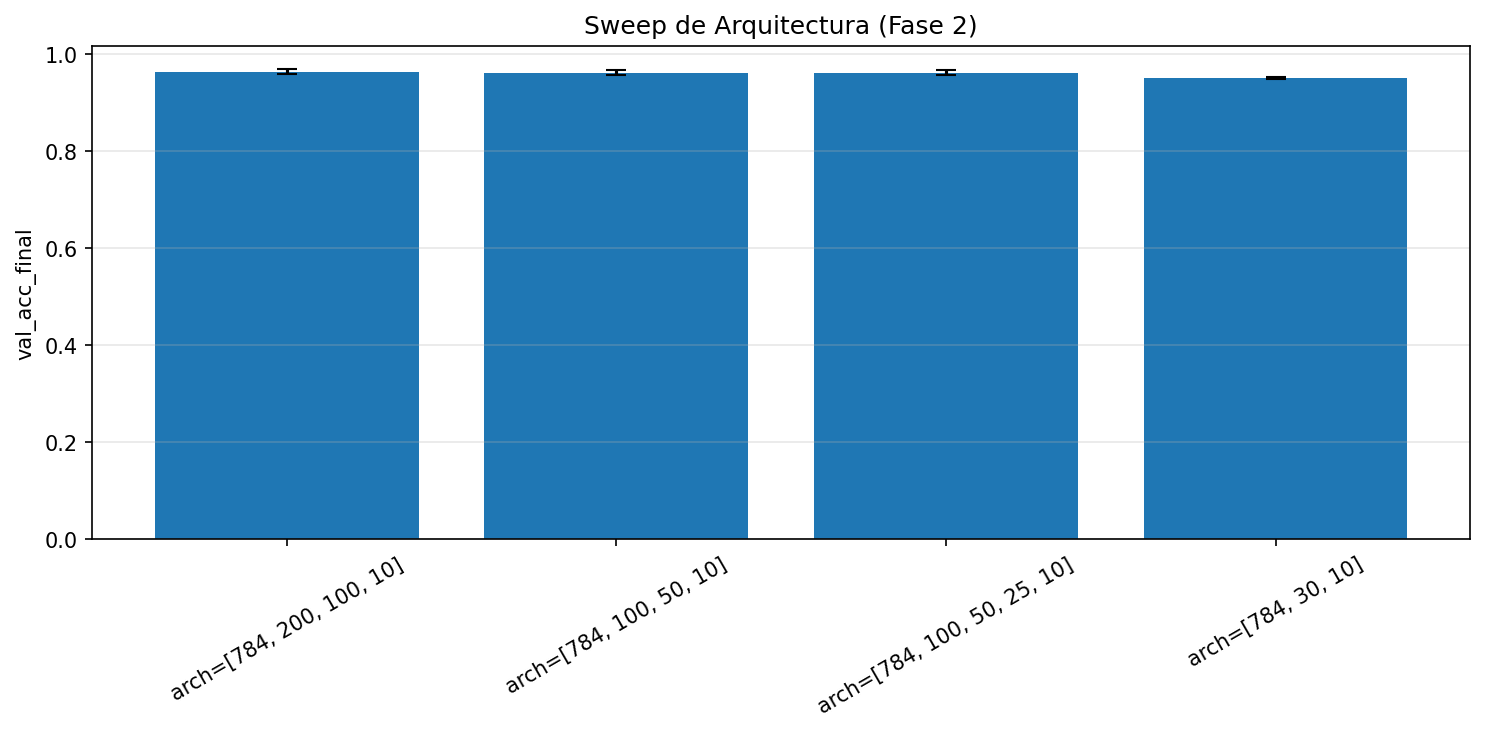
\includegraphics[width=\linewidth]{../ejercicio2/presentacion/03_sweep_arch.png}\\
\textcolor{muted}{\footnotesize Sweep arquitectura — todas en empate}
\end{columns}
\vspace{0.4em}
\begin{insight}
Solo el sweep de LR muestra rangos catastróficos. Arch, opt e init quedan en empate técnico — \textbf{Fase 2 valida más que descubre}.
\end{insight}
\end{frame}

% ============= 17. Curvas + matriz =============
\begin{frame}{Ej 2 — Curvas y matriz del base (val K=5)}
\begin{columns}[T]
\column{0.55\linewidth}
\centering
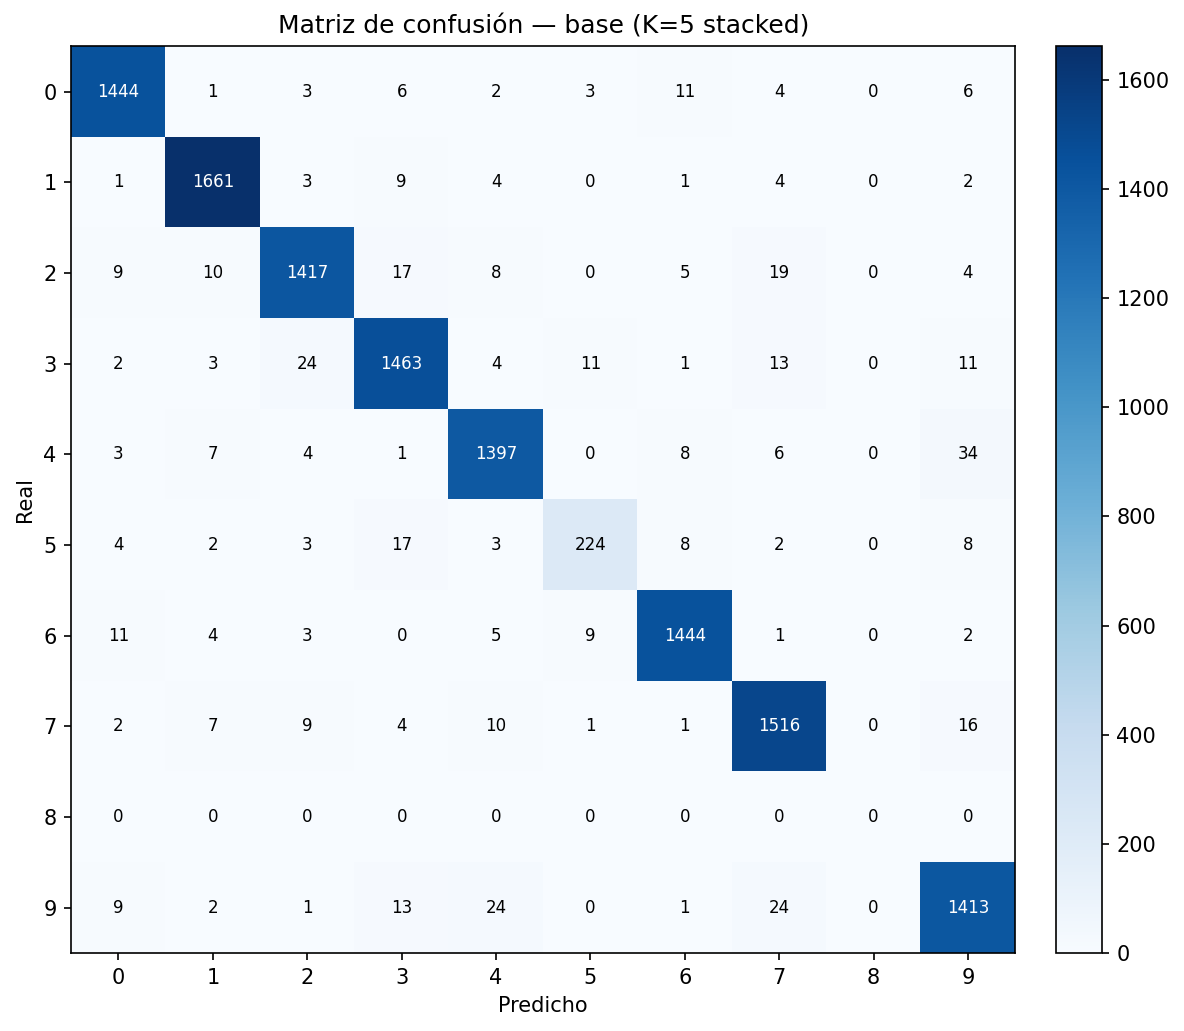
\includegraphics[width=\linewidth]{../ejercicio2/presentacion/04_confusion_matrix_base.png}
\column{0.45\linewidth}
\textbf{Diagonal limpia para 9 de 10 clases.}\\[0.6em]

\textcolor{warn}{\textbf{La clase 8 colapsa:} precision = recall = 0.}\\[0.4em]
\textcolor{muted}{El modelo no la predice nunca en val. Indicador de algo raro en la distribución del train (sub-representación de la clase 8 o ambigüedad en los features).}
\end{columns}
\end{frame}

% ============= 18. Final eval cachetazo =============
\begin{frame}{Ej 2 — Final eval: el cachetazo}
\centering
\vspace{0.6em}
\Huge
val K-fold=5: \textbf{96.22\%}\\[0.5em]
\textcolor{muted}{$\downarrow$}\\[0.5em]
test (digits\_test.csv): \textcolor{warn}{\textbf{86.30\%}}\\[1em]
\Large \textbf{Drop de 10 puntos porcentuales.}\\[1em]

\normalsize
\begin{warning}
\textbf{El modelo está bien — los datos no se parecen.}\\
La matriz de confusión sobre test confirma: las confusiones se reparten por todo el grid, no es una clase específica. Patrón de \textbf{distribution shift}, no de underfitting puntual.
\end{warning}
\end{frame}

% ============= 19. Hipótesis Ej3 =============
\begin{frame}{Ej 2 → Ej 3 — La hipótesis}
\begin{takeaway}
\textbf{Si el problema es shift entre \code{digits.csv} y \code{digits\_test.csv}, no falta de capacidad:}\\
$\Rightarrow$ el primer movimiento debería ser \textbf{más datos}, no un modelo más grande.
\end{takeaway}
\vspace{0.8em}

\textbf{Lo que provee el enunciado del Ej 3:} \file{more\_digits.csv} (15.742 muestras adicionales).\\[0.4em]

\textbf{Lo que el engine ya soporta:} \code{extra\_csv\_paths} en el config concatena CSVs antes del split.\\[0.4em]

\centering\textcolor{muted}{$\to$ \textbf{cero cambios al modelo, solo cambia un campo del JSON}.}
\end{frame}

% ===================================================================
% PERSONA 4
% ===================================================================
\sectiondivider{4 / 4}{Ej 3 — Pack C y conclusiones}

% ============= 20. Plan Ej3 =============
\begin{frame}[fragile]{Ej 3 — Plan}
\textbf{Estrategia secuencial:}\\[0.4em]

\begin{enumerate}
  \item Concatenar \code{more\_digits.csv}. Si \(\geq 0.98\), listo.
  \item Activar Pack C (regularización del enunciado): L2, dropout, augmentation, lr\_schedule.
  \item Si nada llega, escalar capacidad (\code{arch\_wider}).
\end{enumerate}
\vspace{0.6em}

\textbf{Pack C en el engine}: vía campo \code{regularization} del config.
\begin{lstlisting}[language=json, basicstyle=\ttfamily\footnotesize]
"regularization": {
  "l2": 1e-4,
  "dropout": 0.2,
  "lr_schedule": {"type":"step", "decay":0.5, "every":10},
  "augmentation": {"type":"gaussian_noise", "sigma":0.05}
}
\end{lstlisting}
\centering\textcolor{muted}{\footnotesize Implementamos dropout, augmentation y lr\_schedule en \file{mlp/network.py}; tests verde 78/78.}
\end{frame}

% ============= 21. El primer dominó =============
\begin{frame}{Ej 3 — El movimiento dominó}
\centering
\Huge
val K=5: \(96.22\% \to 97.06\%\)\\[0.4em]
test: \textcolor{warn}{\(86.30\%\)} \(\to\) \textcolor{accent2}{\(\boldsymbol{96.36\%}\)}\\[1em]

\Large\textbf{+10 puntos porcentuales en test.}\\
\large\textbf{\textcolor{muted}{Cero cambios al modelo. Solo más datos.}}\\[1em]

\normalsize
\begin{takeaway}
\textbf{Macro F1: $0.857 \to 0.959$.}\\
La clase 8 que estaba colapsada en Ejercicio 2 ahora se predice correctamente. Confirma la hipótesis del shift.
\end{takeaway}
\end{frame}

% ============= 22. Pack C tabla =============
\begin{frame}{Ej 3 — Iteración Pack C}
\centering
\small
\begin{tabular}{@{}lrrr@{}}
\toprule
\textbf{Config} & \textbf{val K=5} & \textbf{test} & \textbf{$\Delta$ vs base\_extra} \\
\midrule
base\_extra\_data            & 0.9706 & 0.9636 & --- (referencia) \\
\quad +\,L2 (1e-4)            & 0.9758 & 0.9656 & $+0.20$ pp \\
\quad +\,dropout (p=0.2)      & 0.9750 & 0.9628 & $-0.08$ pp \\
\quad +\,L2 + dropout         & 0.9772 & 0.9604 & $-0.32$ pp \\
\rowcolor{accent2!15}
\textbf{\quad +\,L2 + aug ($\sigma=0.05$)} & \textbf{0.9760} & \textbf{0.9688} & \(\boldsymbol{+0.52}\)\textbf{ pp} \\
\quad +\,L2 + aug + dropout   & 0.9768 & 0.9656 & $+0.20$ pp \\
\quad +\,wider + L2 + aug     & 0.9777 & 0.9640 & $+0.04$ pp \\
\bottomrule
\end{tabular}\\[0.8em]

\textbf{Ganador:} L2 + augmentation gaussiana ($\sigma=0.05$) $\to$ \textbf{96.88\% en test}.
\end{frame}

% ============= 23. Comparación Ej2 vs Ej3 =============
\begin{frame}{Ej 3 — Comparación visual con Ej 2}
\centering
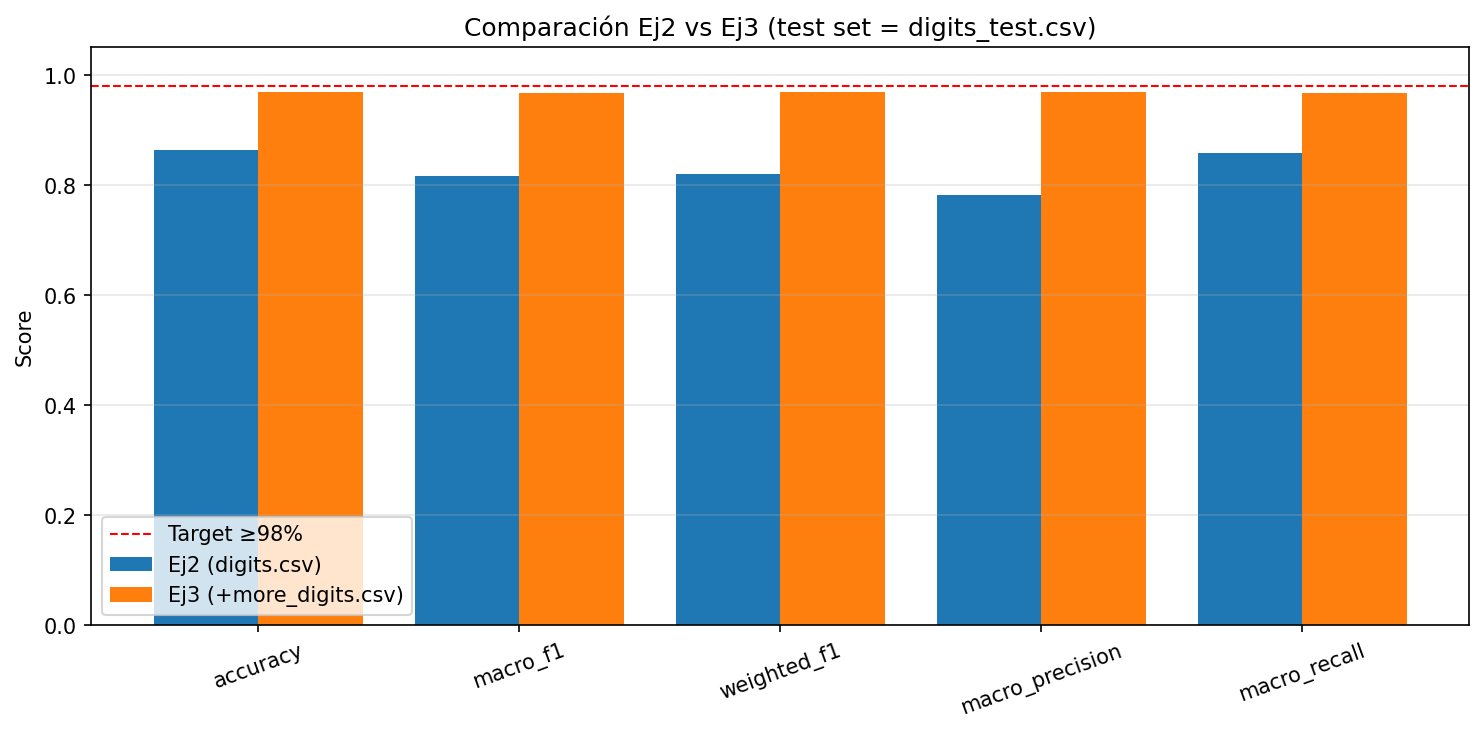
\includegraphics[width=0.78\linewidth]{../ejercicio3/presentacion/01_comparacion_ej2_vs_ej3.png}\\
\textcolor{muted}{\footnotesize Línea roja: target $\geq 98\%$.}
\end{frame}

% ============= 24. Qué movió la aguja =============
\begin{frame}{Ej 3 — Qué movió la aguja}
\begin{insight}
\textbf{Lo que ayudó:}
\begin{itemize}
  \item \textbf{Más datos}: \textbf{+10pp.} El movimiento dominante.
  \item \textbf{L2}: $+0.20$pp consistente.
  \item \textbf{Aug gaussiana}: $+0.32$pp \emph{adicional} sobre L2 (sinergia).
\end{itemize}
\end{insight}

\begin{warning}
\textbf{Lo que no ayudó:}
\begin{itemize}
  \item \textbf{Dropout}: gana en val ($+0.44$pp), pierde en test ($-0.08$pp). Reduce varianza específica al fold, no al shift.
  \item \textbf{wider} \([784,200,100,10]\): mejor en val, peor en test. Más capacidad memoriza, no generaliza. \textbf{Descarta que falte capacidad.}
  \item \textbf{Combinar todo}: L2+dropout+aug peor que L2+aug. La regularización compite consigo misma.
\end{itemize}
\end{warning}
\end{frame}

% ============= 25. Por qué no llegamos al 98 =============
\begin{frame}{Ej 3 — Por qué no llegamos al 98\%}
\centering
\Large \textcolor{warn}{\textbf{Mejor: 96.88\%. Faltan 1.12pp.}}\\[1em]

\normalsize\raggedright
\textbf{Tres hipótesis ordenadas por probabilidad:}
\begin{enumerate}
  \item \textbf{Augmentation insuficiente.}\\
        Gaussian noise es \emph{isotrópico} (independiente por píxel). El shift parece ser de \emph{estilo de escritura}: rotación, traslación, grosor de trazo. Pide augmentation \textbf{geométrica}, no por noise. No la implementamos en este TP.
  \item \textbf{Sub-representación en val interno del final\_eval.}\\
        El final\_eval usa val 10\% random para early stopping. Si los digits ``difíciles'' del test no aparecen ahí, la red para antes de tiempo.
  \item \textbf{Capacidad}: improbable, \code{wider} sobreajustó.
\end{enumerate}
\vspace{0.6em}

\begin{takeaway}
\textbf{Próximo paso}: augmentation por rotación/traslación pequeñas, mantener L2 + $\sigma$ bajo de gaussian noise como rutina, reconsiderar arquitectura solo después.
\end{takeaway}
\end{frame}

% ============= 26. Conclusiones + cumplimiento =============
\begin{frame}{Conclusiones del TP}
\textbf{Tres ideas para llevarse:}
\begin{enumerate}
  \item Una buena pipeline gana más que tunear hiperparámetros: el +10pp del Ej 3 vino de \emph{datos}, no de modelo.
  \item Los empates técnicos son mucho más comunes que los wins claros. Elegir por \textbf{parsimonia}, no por 0.05pp en val.
  \item ``Mejor en val'' \(\neq\) ``mejor en test'' cuando hay shift. Dropout fue el ejemplo: ganador en val K-fold, perdedor en test.
\end{enumerate}
\vspace{0.6em}

\centering\small
\begin{tabular}{@{}lc@{}}
\toprule
\textbf{Item} & \textbf{Status} \\
\midrule
Ej 0 — step AND, MLP XOR, lineal y tanh                    & \ok \\
Ej 1 — Knowledge distillation + threshold sweep             & \ok \\
Ej 2 — MLP from-scratch + sweeps + final\_eval              & \ok \\
Ej 3 — \code{more\_digits.csv} + análisis Pack C             & \ok \\
\textbf{Ej 3 — target \(\geq 98\%\)}                        & \nok\ \textbf{(96.88\%)} \\
\bottomrule
\end{tabular}
\end{frame}

% ============= Cierre =============
{
\setbeamercolor{background canvas}{bg=accent}
\begin{frame}[plain]
\centering
\vspace*{2cm}
\color{white}
{\fontsize{36}{42}\selectfont\bfseries Gracias.}\\[1.5em]
{\Large Preguntas.}\\[2.5em]

\textcolor{white!75}{\rule{6cm}{0.4pt}}\\[1em]
{\small\color{white!75}
\file{github.com/pi-na/SIA-TP3} · branch \code{tp3-mlp}\\[0.3em]
Companion: \file{docs/informe\_tp3.pdf} · \file{docs/guia\_compañeros.md}
}
\end{frame}
}

\end{document}
